\chapter{Grandma Cake / Gateau à Sybil}
\label{ch:grandma_cake}
\index{dessert}
\index{chocolate}
\index{cake}
\textit{Marble bundt cake}

Family member: Metzma Lucie \& Sybil

\marginnote[20pt]{\\
    \textbf{Makes 1 bundt cake} \\
    Prep time: 20 minutes \\
    Cook time: 45 minutes - 1 hour \\
    \vspace*{\baselineskip}

    2 cups sugar \\
    3-4 eggs \\
    1 tsp vanilla extract \\
    3 cups all-purpose flour \\
    3 tsp baking powder \\
    1 cup milk \\
    1 cup vegetable oil \\
    \vspace*{\baselineskip}
    2 tsp cocoa powder 
}
% \newthought{}
% \bigskip

\begin{enumerate}
    \item In a large bowl, whisk the sugar, eggs and vanilla.
    \item In another bowl, whisk the flour and baking powder. Add the dry ingredients to the sugar/egg mixture above in 2 times.
    \item Add the milk, then once completely incorporated, add the oil.
    \item Place half of the mix in a separate bowl, and sift in the cocoa powder. Mix it well.
    \item Grease a loaf pan and line with parchment. 
    \item Pour the chocolate mix in the pan, then the vanilla. Use a knife to swirl both mixes.
    \item Bake at 350\degree F for 45 minutes to 1 hour.
\end{enumerate}

\begin{figure}
  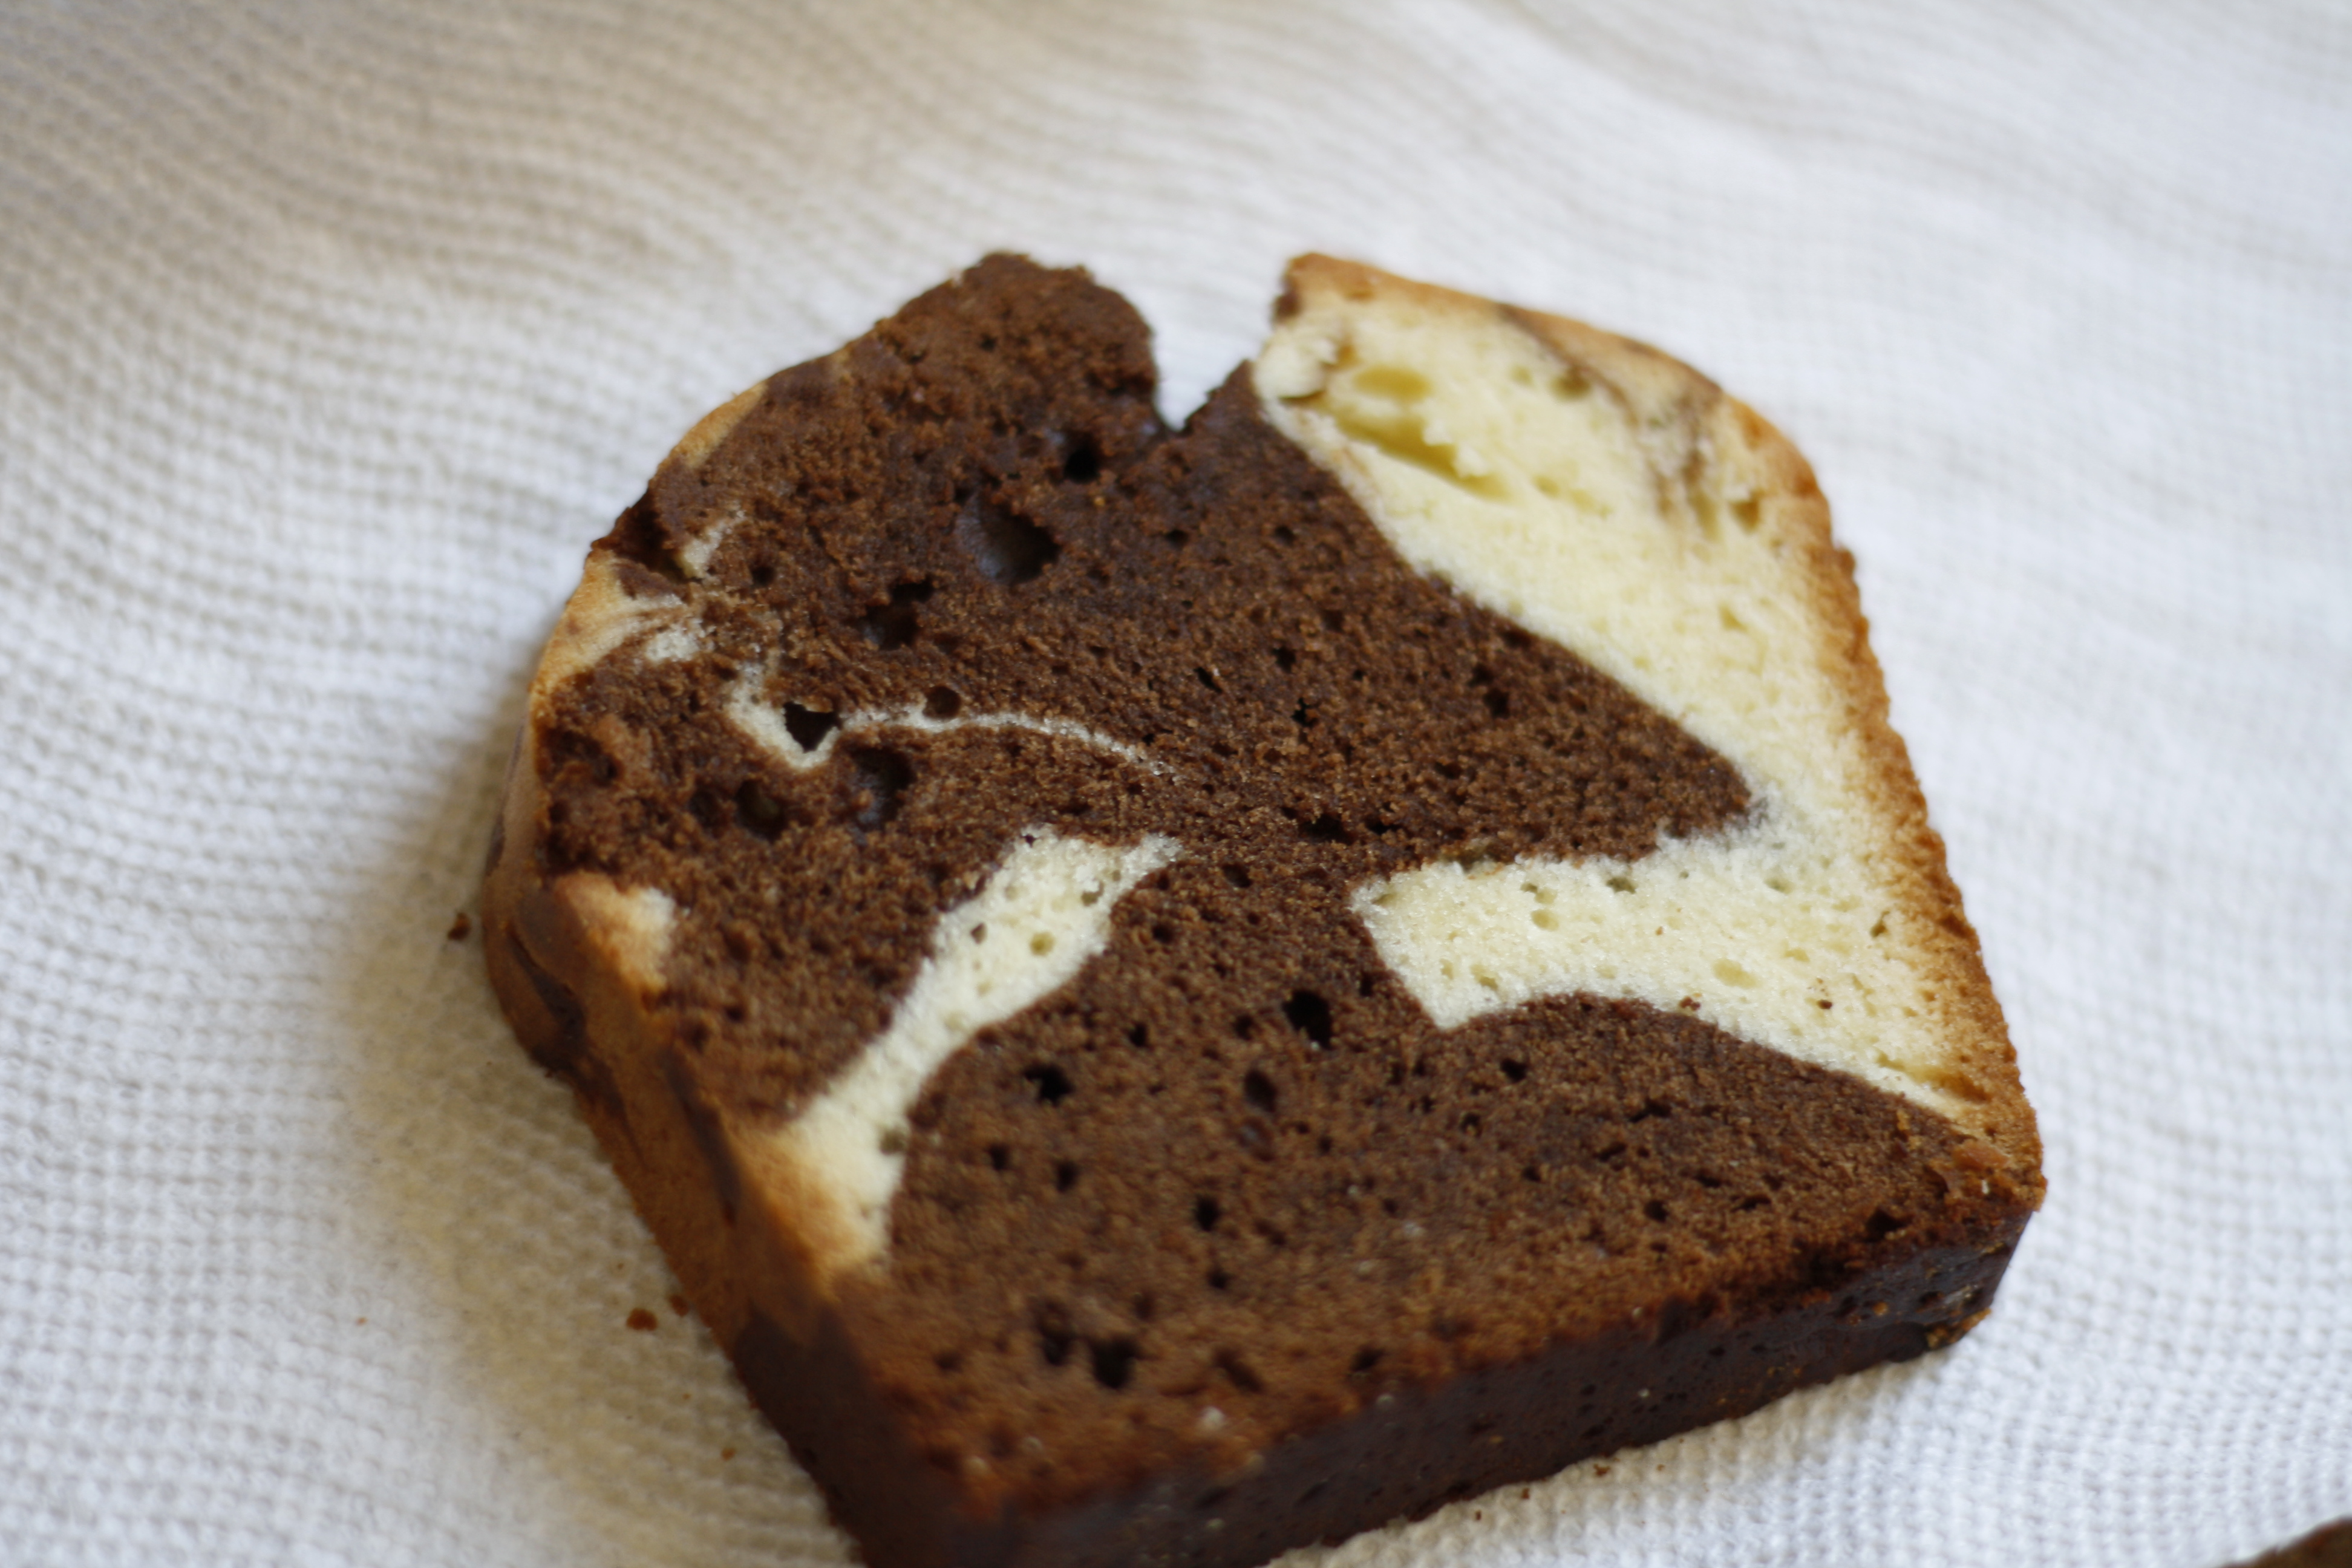
\includegraphics[width=60mm]{dermardiros/images/Grandma cake 1.JPG}
  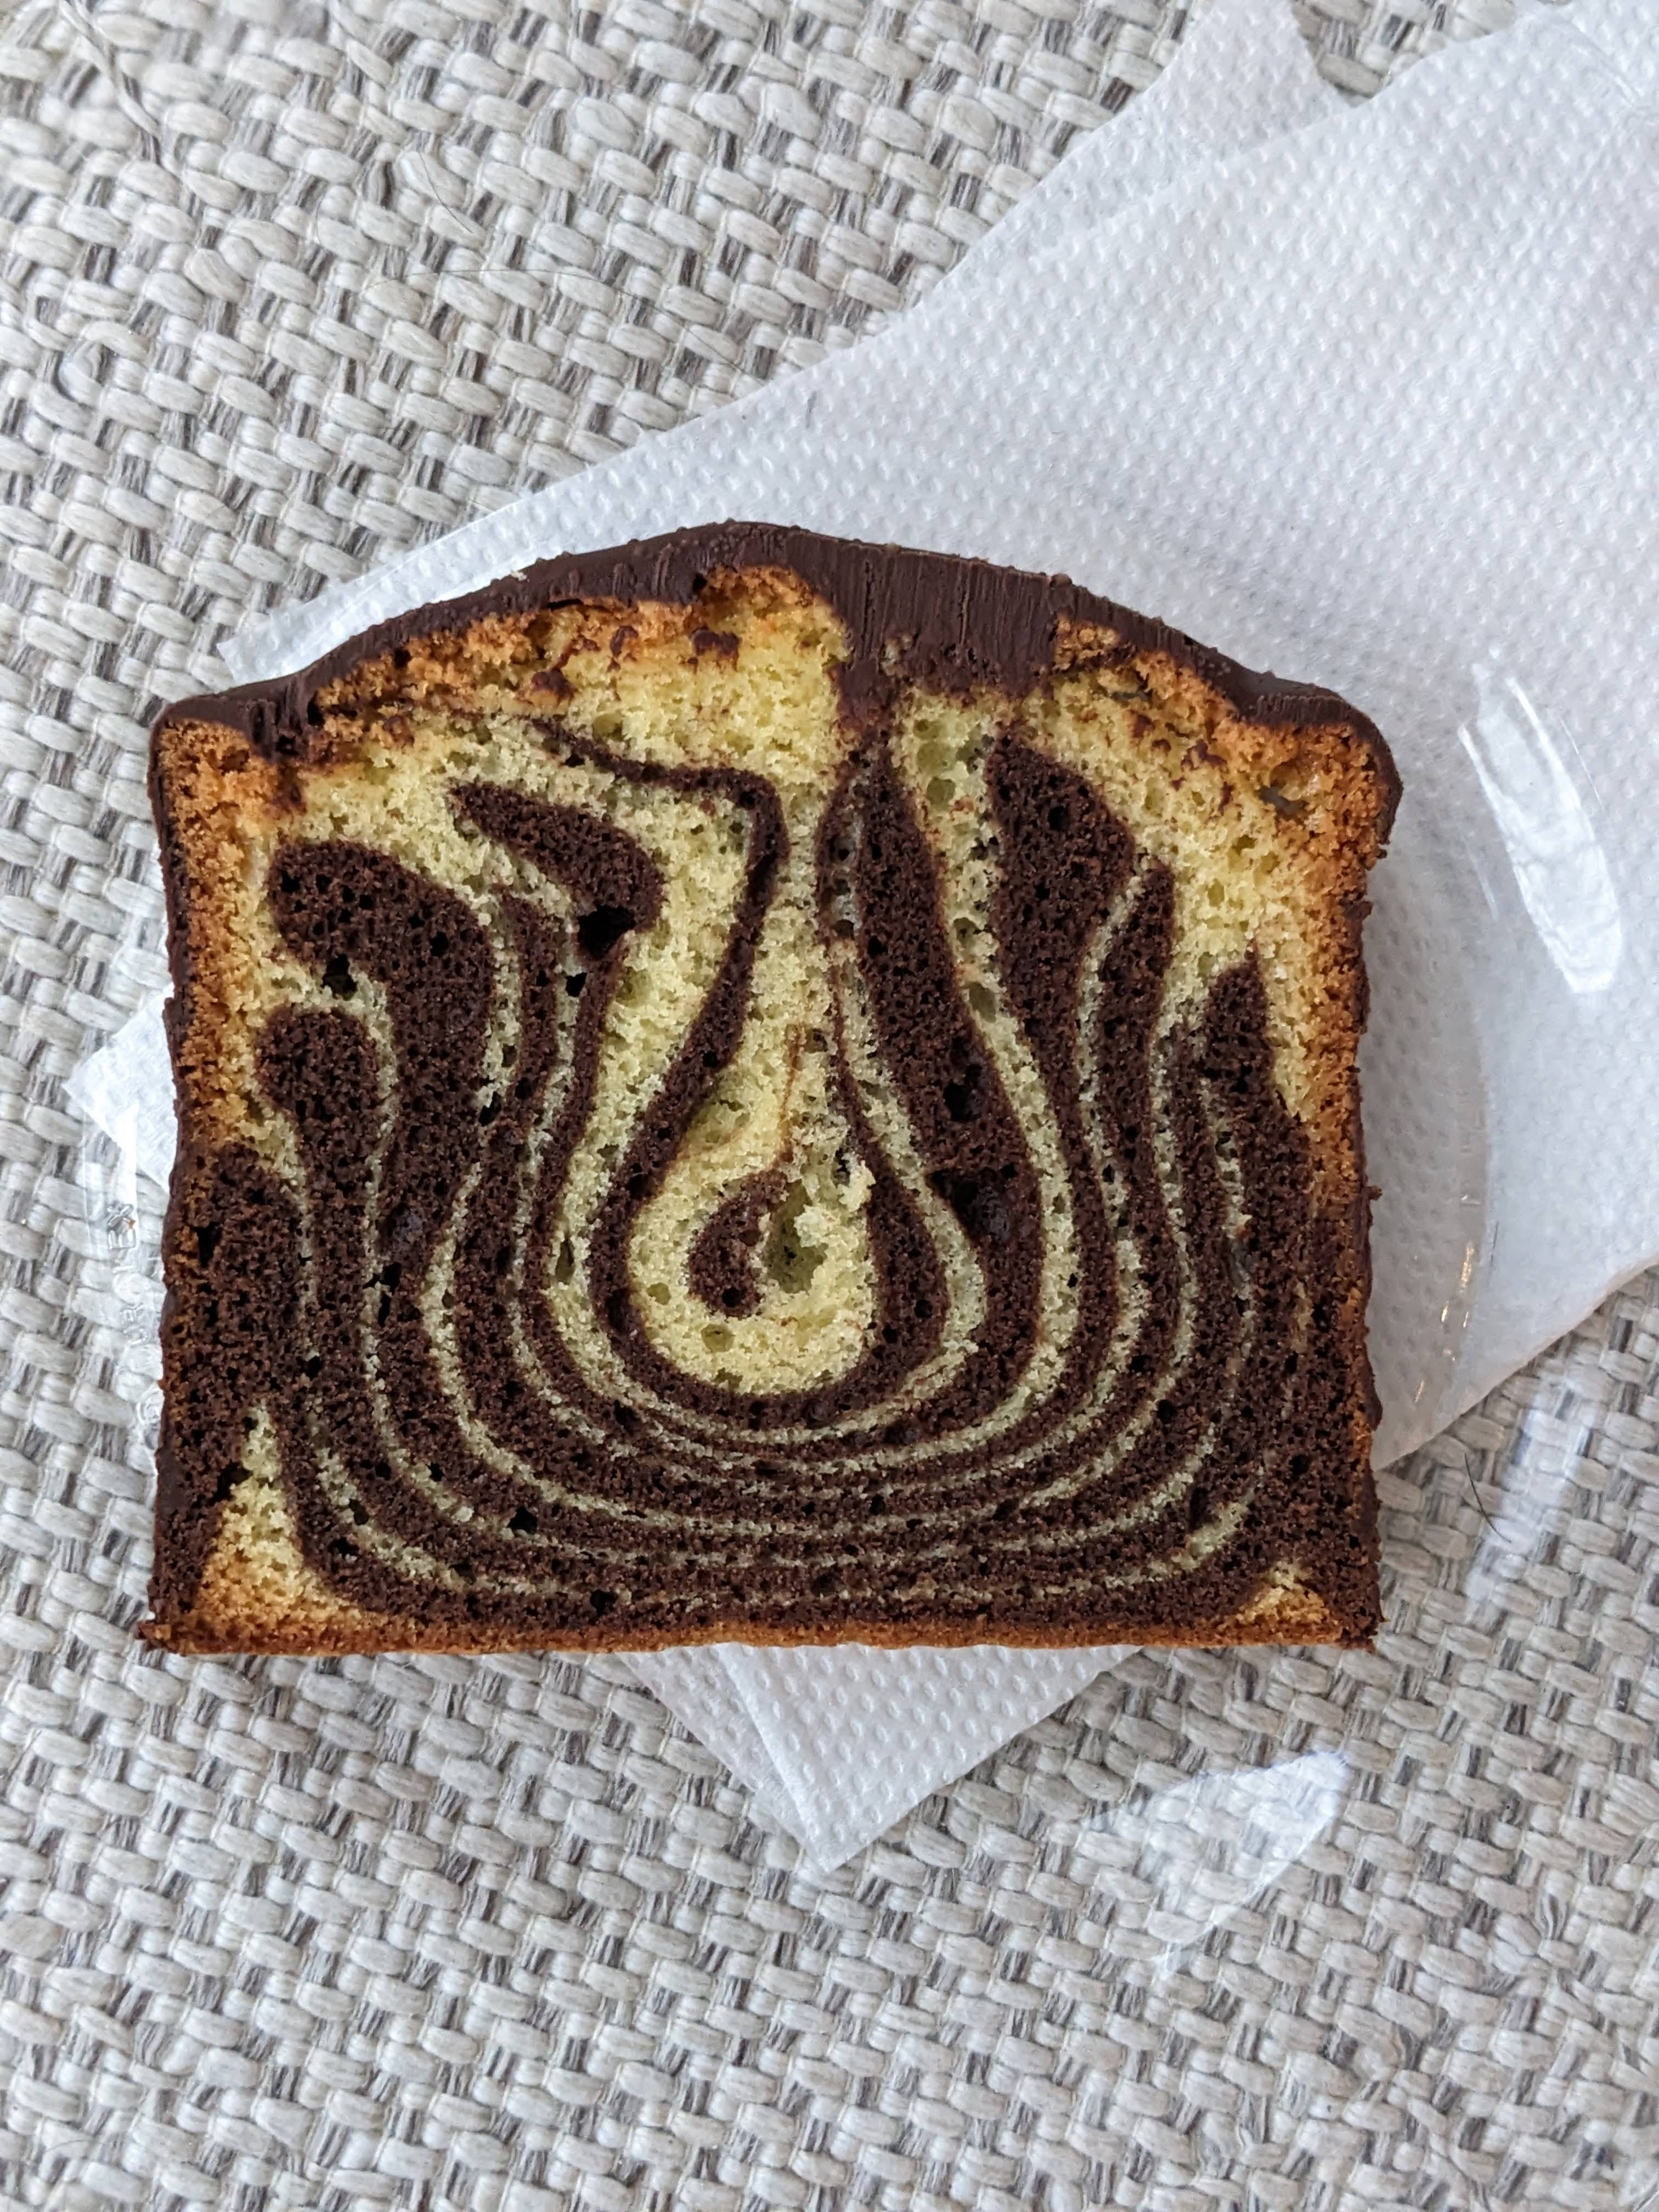
\includegraphics[width=50mm]{dermardiros/images/Grandma cake 2.jpg}
\end{figure}

\marginnote{
    Sybil’s alternatives: orange zest and 1 cup chocolate chips, 2 bananas, 1 cup raisins… You can use more cocoa powder if you want to have a deeper chocolate taste.
}